\chapter{Teil 1: Gold Standard}
\section{Vorgehen}
Als Rohdaten zur Erhebung dieses Gold Standards dient der Output des Webcrawlers.
Die Erarbeitung dieser Rohdaten kann im \cref{chap:engineering} nachgelesen werden.\\
\subsection{Erarbeitung des Entscheidungsrasters}
Das Entscheidungsraster ist die Grundlage des manuellen Labeling der Rohdaten.
Für dieses wurden die folgenden Entscheidungen getroffen:
\begin{itemize}
	\item Die Webpage muss auf Deutsch verfasst sein
	\item Der Anbieter muss entweder ein Restaurant, Take-Away oder Lieferdienst sein
	\item Der Text muss statisch im HTML vorhanden sein, da dynamisch gerenderte Informationen vom Webcrawler nicht gespeichert werden
	\item Es muss ein Menü, also eine Kombination aus mehreren Speisen oder eine einzelne Speise vorhanden sein
	\item Eine genauere Beschreibung oder der Preis muss vorhanden sein
	\item Getränkekarten werden explizit als negativ gelabelt
\end{itemize}
Bei der Klassifizierung wird zudem unterschieden, ob es sich um ein zeitlich begrenztes Angebot handelt, da diese Angebote zu einem späteren Zeitpunkt eventuell zusätzlich erkannt werden möchten.
\subsection{Manuelles Labeling der Daten}
In einer ersten Durchführung des manuellen Labelings wurden ca. 1500 Dateien klassifiziert, welche das Schlüsselwort \glqq Menu\grqq{} in der URL enthalten.
Die mit dieser Heuristik gefilterten Daten entsprechen jedoch nicht einer repräsentativen Teilmenge der gesamten Rohdaten.
Darum wurde in einer zweiten Durchführung zufällig Proben aus den Rohdaten ausgewählt und manuell gelabelt.
Dadurch konnte sichergestellt werden, dass das Verhältnis von Menüseiten zu den restlichen Webpages gleich bleibt.
\subsection{Hilfsmittel: Labeling-Tool}
Um das manuelle Labeling effizienter zu gestalten, ist ein Tool\footnote{\url{https://github.com/s-santoro/testdata_tool} abgerufen am: 11.03.2019} erstellt worden, welches das Labeling vereinfacht.
Dieses Tool ruft eine Webpage der zufällig extrahierten Webpages aus den Rohdaten auf und zeigt sowohl den Text, als auch den HTML-Inhalt.
Der Anwender des Tools muss anhand dieser Informationen entscheiden, ob es sich um eine Webpage mit Menüinformationen handelt und ob diese zeitlich begrenzt sind.
Mittels Shortkeys findet die Klassifizierung statt.
Das Tool verschiebt die Datei in den entsprechenden Ordner und zeigt die Informationen der nächsten Webpage an.
\section{Seed}
Das Seed wurde als Datenquelle des Webcrawlers verwendet und bildet somit die Grundlage dieses Gold Standards.
Es wurde aus den folgenden zwei Quellen zusammengestellt:
\begin{itemize}
	\item OpenStreetMap - 3557 URLs
	\item Lunch-Check - 3803 URLs
\end{itemize}
Diese Quellen wurden verwendet, da sie diese Daten für diese Arbeit kostenlos zur Verfügung stellen.
Die URLs wurden zusammengeführt und Duplikate sind entfernt worden.
Daraus ist ein Seed entstanden, welches 5870 Einträge von Restaurant-URLs enthält.
Dabei wurden aus den nun aufgeführten Gründen mehrere Einträge entfernt:
\begin{itemize}
	\item Die Website enthält mehr als 300 Webpages
	\item Die Website ist offensichtlich keine Restaurant-Website
\end{itemize}
Websites mit mehr als 300 Webpages wurden entfernt, da diese keine typische Restaurant-Website repräsentieren und somit das Gesamtbild verzerren.
Es kann keine Gewähr gegeben werden, dass dieses Seed nur Restaurant-Websites beinhaltet, da nicht jeder Eintrag geprüft wurde.
\section{Entscheidungsraster}
\FloatBarrier
Der Gold Standard wurde anhand des Entscheidungsrasters erstellt, welches in der \cref{fig:classificationtree} dargestellt wird.
\begin{figure}	
	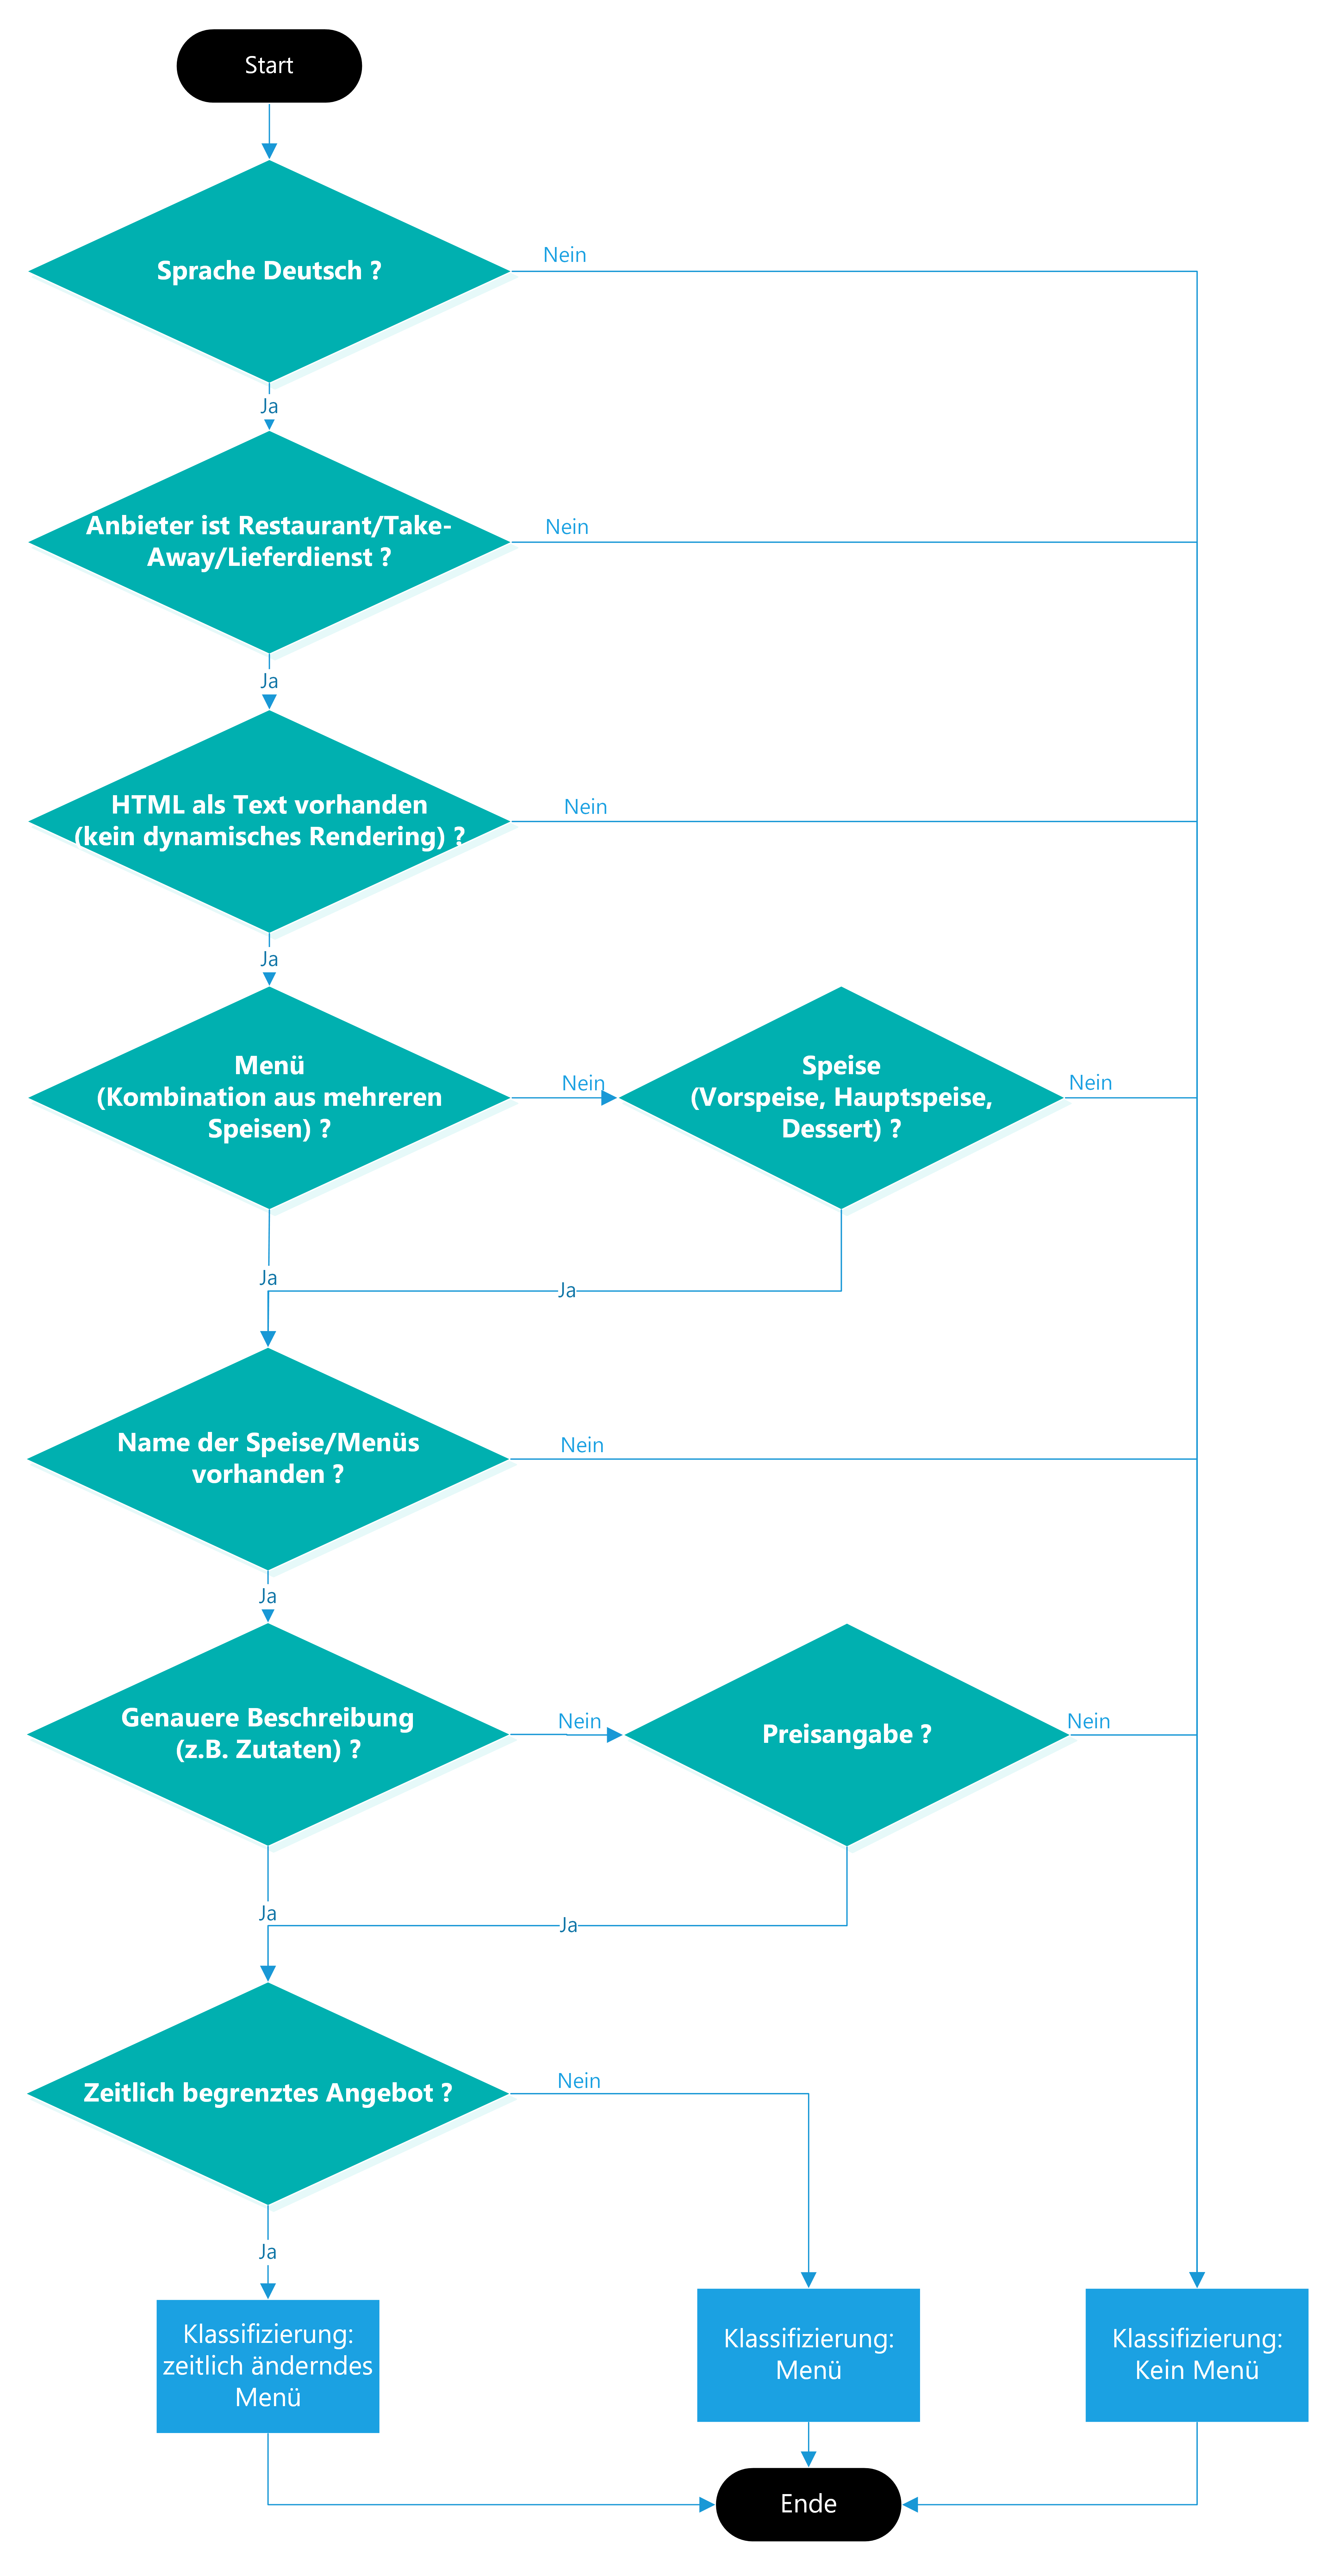
\includegraphics[width=0.65\columnwidth,keepaspectratio]{img/man-classification-tree.png}
	\caption{Entscheidungsraster}
	\label{fig:classificationtree}
\end{figure}
Obwohl bereits beim Webcrawler eine Spracherkennung eingesetzt wurde, damit nur als deutsch erkannte Webpages gespeichert werden, wurde bei der manuellen Klassifikation nochmals darauf geachtet, dass die Webpage in deutsch verfasst wurde.
Dabei ist anzumerken, dass gewisse Begriffe, vor allem für Speisebezeichnungen, auch fremdsprachig sein dürfen, da Speisebezeichnungen je nach Küche international ausgelegt sind.
Der Anbieter muss zwingend ein Restaurant, Take-Away oder Lieferdienst sein.
Der Inhalt muss statisch in der HTTP-Antwort verfügbar sein, da der Webcrawler nur diesen speichert und nicht mit dynamisch gerenderten Websites umgehen kann.
Der Name der Speise und eine genauere Beschreibung oder der Preis muss vorhanden sein.
Danach folgt die Unterscheidung zwischen zeitlich begrenzten und unbegrenzten Angeboten, welche zur Kategorisierung führt.
Getränkekarten wurden explizit negativ klassifiziert.
\FloatBarrier
\section{Beschreibung des Gold Standards}
Der erarbeitete Gold Standard besteht insgesamt aus 6963 Dateien des Formats JSON, welche jeweils eine Webpage einer Restaurant-Website repräsentieren.
Diese Daten sind in einen Test- und einen Trainings- und Validierungsdatensatz unterteilt.
Der Gold Standard beinhaltet die folgenden drei Kategorien:
\begin{itemize}
	\item neg $\rightarrow$ Kein Menü
	\item pos\textunderscore daily\textunderscore menu $\rightarrow$ Zeitlich änderndes Menü
	\item pos\textunderscore menu $\rightarrow$ Menü
\end{itemize}
Die Datenstruktur des Gold Standards sieht wie folgt aus:\\

\begin{forest}
	for tree={
		font=\ttfamily,
		grow'=0,
		child anchor=west,
		parent anchor=south,
		anchor=west,
		calign=first,
		edge path={
			\noexpand\path [draw, \forestoption{edge}]
			(!u.south west) +(7.5pt,0) |- node[fill,inner sep=1.25pt] {} (.child anchor)\forestoption{edge label};
		},
		before typesetting nodes={
			if n=1
			{insert before={[,phantom]}}
			{}
		},
		fit=band,
		before computing xy={l=15pt},
	}
	[Gold Standard (6963 Dateien)
	[test (100 Dateien)
	[neg (50 Dateien)]
	[pos\textunderscore daily\textunderscore menu (10 Dateien)]
	[pos\textunderscore menu (40 Dateien)]
	]
	[train-validation (6863 Dateien)
	[neg (6257 Dateien)]
	[pos\textunderscore daily\textunderscore menu (87 Dateien)]
	[pos\textunderscore menu (519 Dateien)]
	]
	]
\end{forest}\\


Jeder Eintrag dieses Gold Standards beinhaltet die folgenden Informationen:
\begin{itemize}
	\item \glqq date\grqq{} - Zeitpunkt, zu welchem die Webpage aufgerufen wurde
	\item \glqq text\grqq{} - Vom Webcrawler extrahierter Text, welcher die Webpage beinhaltet
	\item \glqq encoding\grqq{} - Das von der Webpage verwendete Encoding
	\item \glqq title\grqq{} - Inhalt des gleichnamigen HTML-Metatags
	\item \glqq url\grqq{} - URL der Webpage
	\item \glqq content\grqq{} - Der statische HTML-Inhalt der Webpage	
\end{itemize}


